Here we describe three stopping algorithms for sequential hypothesis testing.

We begin by describing heuristics of posterior location and width used in all three.
We describe their intuition, as well as in pseudo code.
We also provide useful anlaytical experessions and conclude by describing a setup
to test the methods on synthetic data.
Although our belief is that these methods apply to any type of data,
our focus is on dichotomous data (Bernouli trials)
in order to compare with \cite{kruschke2015doing}
(somehow experess that: "as it is simple to describe analytically and
to conduct rapid tests on synthetic data.")


We conclude with a contrast comparison of the algorithms.

(Mention somewhere difference between "stopping algorithm" to "stopping criterion",
perhaps "collection algorithm"?)


\subsubsection{Region of Practical Equivalence and High Density Interval}
All three stop algorithms explored below depend on heuristics that describe two key
aspects of expectations from the experiment:
\begin{itemize}
    \item Effective size expected from the experiment
    \item Posterior width
\end{itemize}


One common misconception in hypothesis testing is that an outcome that is
“statistically significant” is sufficient to make a meaningful real world decision.
In practice one must consider the effect size.
E.g, medical research requires a “minimal detectable change” or
“minimal clinically important difference” to consider an outcome relevant for
considering a change in action.

As an over simplistic made-up example imagine that a researcher examines if a
therapeutic differs in impact by gender.
If we assume that enough data was collected to demonstrate that the difference is
“statistically significant”, e.g, that the drug is 72.1\% beneficial for males
and 72.3\% for females, a practitioner, depending on circumstance may consider
this equivalent for all practical purposes.
To justify treating the usage of the drug by gender the
researcher (or the board of the company or a regulatory body) would demand
a meaningful absolute difference e.g,  5\% or 10\% or more
(depending on the context, e.g, for purposes of further research, or approval
of the drug). Hence the researcher should define in advance of collecting data an
“effective area" around the null hypothesis being examined to determine if a
decision making difference is present.

One such metric of interest to account for the importance of the effective size
is referred to as the
\textit{Region of Practical Equivalence} (ROPE).
The ROPE is defined as an area around the null value considered “similar enough 
to the null hypothesis" such that if the true value is within this area by all
means it is effectively the same to the null hypothesis.

The width of the ROPE depends on the task at hand.
E.g, consider the precision of the fairness of dice required in a family board game
against that required for gambling enterprises.
A manufacturer of household board games would like them to be fair to a certain extent,
but would not want to pay a premium for accuracy that would not be noticed by a casual
player. A casino on the other hand would require a much higher accuracy to ensure
players that the dice are not loaded.

In the algorithms expolred here we are intersted in the quantifying the overlap
between the posterior and the ROPE, e.g a \textit{credible interval} (similar to the frequentist confidence interval).
A popular heuristic is the \textit{Highest Density Interval} (HDI)
which describes the region where a substantial amount of the posterior resides.
In practice the HDI means that all points within the credible interval have a higher
probability density than points outside of it.

The width of the HDI is commonly calculated using 95\% of the mass to be comparable
with that used traditionally in Frequentist hypothesis testing.
Whereas this is reasonable for analytical solutions (i.e, solved using an equation),
for numerical solutions it has been shown that for high precision 10,000 samples are
required, otherwise one should use a lower mass percentage like 94\% (Kruschke, 2014, look up BIB).
\cite{mcelreath2016} suggests 89\% as a quip to the arbitrariness of the importance of the
width of the credible interval, where the only noteworthy feature of this value is being
the highest prime value under the traditional 95\% threshold.  

The ROPE and HDI metrics may be used in various combinations in the
test criterion algorithm.
The three algorithms explored here differ in their stop criterion, which we later
details, but have the same decision criterion which we discuss next.


\subsubsection{Decision Criterion: Is The HDI In Or Out Of The ROPE?}\label{sec:decision_criterion}

\begin{figure}[h!]
    \centering
    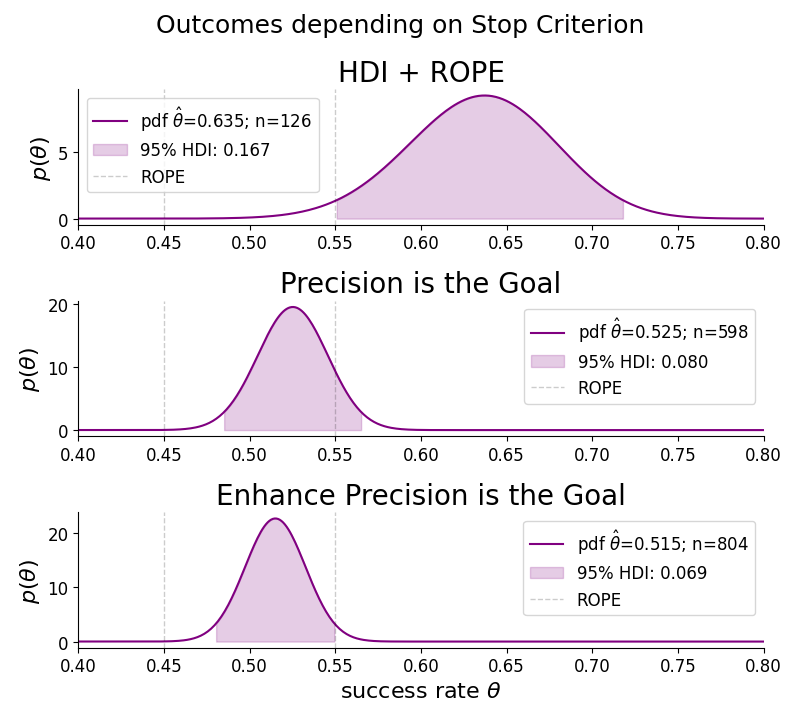
\includegraphics[width=1\textwidth]{cherry_posteriors.png}
    \caption{Posteriors of subsamples of an example sequence. (For the full sequence see Figure TBD.)
    In each panels is the posterior for a different stop criteria being triggered as per panel titles.
    Shaded areas are 95\% HDIs. The ROPE within vertical dashed lines.
    The outcome is dependent on when the stop criterion is triggered.
    Top - HDI fully outside of ROPE → rejects $\theta_{\rm null}$.
    Middle - HDI straddles ROPE → Inconclusive.
    Bottom - HDI fully within ROPE → Accept $\theta_{\rm null}$.
    %Top - HDI+ ROPE triggers when the 95\% HDI is fully outside the ROPE (iteration 126). Incorrectly rejects $\theta_{\rm null}$. Middle - “Precision is the Goal” triggers when 95\% HDI width reaches precision goal of 80\% ROPE width (iteration 598). HDI straddles the ROPE → inconclusive.
    %Bottom - “Enhanced Precision is the Goal” triggers when 95\% HDI fully within ROPE and obtains same precision goal (iteration 804). Correctly accepts $\theta_{\rm null}$
    }
    \label{fig:posteriors}
\end{figure}

Once the stop criterion is triggered (be it manual or automated),
the decision criterion for all three algorithms discussed is as follows:

\begin{itemize}
    \item If the HDI is completely outside ofthe ROPE → Reject the Null Hypothesis
    \item If the HDI is completely inside the ROPE → Accept the Null Hypothesis
    \item Otherwise → Inconclusive
\end{itemize}

We emphasise the third option of “inconclusive” as when the HDI straddles the ROPE
boundaries. Addressing the issue of too many inconclusive outcomes is the main contribution of this study.

In Figure \ref{fig:posteriors} we show three different posteriors of the same experiment of Bernoulli
trials (i.e, same sample of coin tosses). % of a fair coin ($\theta_\mathrm{true}$=0.5).
Each panel shows the posterior of a subsample when a different stopping iteration
%criterion algorithm would have been triggered as mentioned in the title.
The posterior used is the Beta distribution which quantifies $P(\theta|\hat{\theta})$,
i.e the probability that a
success rate $\theta$ (the horizontal axis) to generate this subsample,
given we observed the subsample mean $\hat\theta$ (no. of successes/no. of tosses)
as quantified in the legend of each panel.

In the top panel we examine the posterior
%of the \textit{HDI+ ROPE} algorithm (defined below)
when stopped at iteration 126 when the 95\% HDI is fully outside the ROPE.
In this case the algorithm %incorrectly
rejects the null hypothesis $\theta_{\rm null}$.

In the middle pannel we see the posterior
%of the \textit{Precision is the Goal} algorithm (defined below).
when a stop criterion was triggered at iteration 598
%when the 95\% HDI width achieved the precision goal of 0.08 (80\% of the ROPE width).
In this case the HDI straddles and the decision is inconclusive.

In the bottom panel we see the result
%of the \textit{Enhanced Precision is the Goal} algorithm
when stopping at iteration 804.
Since the 95\% HDI is fully within the ROPE
%and achieved the same goal precision.
%In this case it correctly accepts
$\theta_{\rm null}$ may be accepted (TBD: J.K's comment about only central value).

The main insight from this Figure \ref{fig:posteriors} (which is based on a 
cherry picked example) is that the decision outcome may would be differ by iteration.
More data, obviously is better, but the main question is when is best stop.
\\
\\
Alternative Text that focuses on the main insight and does not mention the algorithms:\\


In the top panel we see that in trial 126 the HDI is completely outside of the ROPE.
If the stop criterion is triggered the user would reject the null hypothesis.
In the middle panel we see that at trial 598 the posterior straddles the ROPE.
If the stop criterion has not been triggered the researchers would need to collect more
data. If it has been triggered, the result is inconclusive and the researcher would have
to use other mechanisms to assess the risk of accepting or rejecting. In the bottom
panel at trial 804 the HDI is fully within the ROPE. If the stop criterion is triggered
here the null hypothesis is correctly accepted. The main insight from this figure is
that in all three stopping criteria the decision would be different.

\subsubsection{A High Level Comparison Of The Three Algorithems}

As mentioned above, when the stop criteria trigger, all three test algorithms
apply the same decision criterion but in slightly different manners.


Table \ref{tab:table1} provides a high level comparison between the test algorithms.


\begin{table}[h!]\label{tab:table1}
    \begin{center}
      %\caption{Multirow and -column table.}
      \begin{tabular}{c|c|c|c}
        \textbf{Test Algorithm } & \textbf{Pre Survey} & \textbf{Stop Criterion} &  \textbf{Decision Criterion}\\
        \hline
        HDI + ROPE & $N_\mathrm{min}$  & \multicolumn{2}{c}{\multirow{1}{*}{HDI within/outside ROPE?}}  \\
        Precision is the Goal & Goal & Precision $<$ Goal? & HDI within/outside ROPE? \\
        Enhanced Precision is the Goal & Goal& \multicolumn{2}{c}{\multirow{1}{*}{(Precision $<$ Goal?) \& (HDI within/outside ROPE?)}}  \\
      \end{tabular}
      \caption{A high level comparison between the test algorithms.
      The merged cells mean Stop and Decision criteria are simultaneous.
      Otherwise multi-step.
      }
    \end{center}
  \end{table}

In the Pre Survey column we highlight the a characteristic parameter required to be
determined prior to the collection of data. For HDI+ROPE this is the minimal sample size
to collect $N_\mathrm{min}$, e.g, 30. The reason for this is that this algorithm
is very sensitive to strong outliers.

For the two precision based algorithms the $\mathrm{GOAL}$ precision is required,
which should be less than the $\mathrm{ROPE}$ width $\Delta_\mathrm{ROPE}$. For brevity of the table
readability we excluded two Pre Survey parameters that are required for all three
algorithms:
\begin{itemize}
    \item $N_\mathrm{max}$ - the maximum sample size, i.e, the final budget size. In most practical cases one will want an upper bound of how much data to collect
    \item $\Delta_\mathrm{ROPE}$ - The ROPE width which is a statement of minimum effect size considered meaningful
\end{itemize}

In the Stop and Decision Criteria columns we see that,
as per \S\ref{sec:decision_criterion}, the decision criterion is the same
for all three. That is to say that all three make the decision based on the
location of the HDI with respect to the ROPE, i.e, the posterior location in respect
to the null hypothesis and its effective region.
Whereas this is the only criterion for the HDI+ROPE algorithm, the other two
are more conservative as they require also the posterior width information in the from
of what is later to be defined as the Precision.

\begin{algorithm}
    \caption{Decision Criterion pseudo algorithm}\label{alg:decision_criterion}
    \begin{algorithmic}
    \Require $\mathrm{ROPE}_\mathrm{min}$, $\mathrm{ROPE}_\mathrm{max}$, $\mathrm{HDI}_\mathrm{min}$, $\mathrm{HDI}_\mathrm{max}$
    \If{$(\mathrm{ROPE}_\mathrm{min} < \mathrm{HDI}_\mathrm{min}) \ \& \ (\mathrm{HDI}_\mathrm{max} < \mathrm{ROPE}_\mathrm{max})$}
        \State Decision = Accept $\theta_{\rm null}$ \Comment{HDI completely within ROPE}
    \ElsIf{$\mathrm{ROPE}_\mathrm{max}<\mathrm{HDI}_\mathrm{min}$}
        \State Decision = Reject $\theta_{\rm null}$ \Comment{HDI completely outside ROPE; $\theta_{\rm null}<\hat\theta$}
    \ElsIf{$\mathrm{HDI}_\mathrm{max}< \mathrm{ROPE}_\mathrm{min}$}
        \State Decision = Reject $\theta_{\rm null}$ \Comment{HDI completely outside ROPE; $\hat\theta<\theta_{\rm null}$}
    \Else
    \State Decision = Inconclusive  \Comment{HDI straddles ROPE}
    \EndIf \\
    \Return Decision
    \end{algorithmic} 
    
\end{algorithm}


Note that the Precision is the Goal method is a two step process, 
i.e, "Stop" then "Decide",
and the other two activate both Stop and Decision criteria simultaneously
(i.e, "Stop and Decide"). In the next three secions we explain these in detail,
followed up with analytic and synthetic examples.


\subsubsection{HDI + ROPE: Location, Location, Location}

HDI + ROPE is a popular method that combines the HDI and ROPE heuristics to describe
the relationship between the \textbf{location} of posterior $P(\theta|\hat\theta)$, which depends on the observed
sample value $\hat\theta$ in regards to the
null hypothesis $\theta_{\rm null}$.

In Algorithm \ref{alg:hdi_rom} we provide a pseudo code of the HDI + ROPE algorithm.

\begin{algorithm}
    \caption{HDI + ROM pseudo algorithm}\label{alg:hdi_rom}
    \begin{algorithmic}
    \Require $N_\mathrm{min}$, $N_\mathrm{max}$, $\theta_{\rm null}$, $\Delta_\mathrm{ROPE}$
    \State $\mathrm{ROPE}_\mathrm{min} = \theta_{\rm null} - \frac{1}{2}\Delta_\mathrm{ROPE}$
    \State $\mathrm{ROPE}_\mathrm{max} = \theta_{\rm null} + \frac{1}{2}\Delta_\mathrm{ROPE}$
    \State Decision = Inconclusive
    \State Stop = False
    \State N = 0
    \While{(Stop = False \& $N \le N_\mathrm{max}$)}  % perhaps change to while loop
    \State N += 1 \Comment{collect another data point} 
    \State Update $\hat\theta$, $P(\theta|\hat\theta)$ \Comment{update posterior} 
    \State $\mathrm{HDI}_\mathrm{min}, \ \mathrm{HDI}_\mathrm{max}  \gets P(\theta|\hat\theta)$
    \If{$N < N_\mathrm{min}$}
         \State pass  \Comment{collect more data without testing for Decision}
    \ElsIf{$N_\mathrm{max} < N $} \Comment{Reached the maximum sample size}
        \State Stop = True  
        \State Decision = Inconclusive    
    \Else
        \State Decision = Decision Algorithm($\mathrm{ROPE}_\mathrm{min}, \mathrm{ROPE}_\mathrm{max}, \mathrm{HDI}_\mathrm{min}, \mathrm{HDI}_\mathrm{max}$)
        \If{Decision in \{Accept $\theta_{\rm null}$, Reject $\theta_{\rm null}$\}}
            \State Stop = True  \Comment{Stopping only when decisive decision}
        \EndIf
    \EndIf
    \EndWhile
    \end{algorithmic}
\end{algorithm}


The algorithms requires a few decisions to be made prior to the collection of data (Pre Survey Decisions):

\begin{itemize}
    \item $N_\mathrm{min}$ - the minimal sample size to collect
    \item $N_\mathrm{max}$ - the maximum sample size
    \item $\theta_{\rm null}$ - the null hypothesis parameter value being tested
    \item $\Delta_\mathrm{ROPE}$ - The ROPE width (minimum effect size)
\end{itemize}

Algorithm \ref{alg:hdi_rom} assumes collection of one data point at a time,
but this may be modified in the line $N += 1$ to be for a batch collection.

The most important aspects of this algorithm are that:

\begin{itemize}
    \item The Stop and Decision criterion are one and the same
    \item The Stop criterion depends only on location information, not on the precision of the posterior.
\end{itemize}

Due to its disregard of dependence on the uncertainty of the posterior,
this popular method serves as a cautionary use case of the "confirmation bias"
address by the Precision based methods described next.


\subsubsection{Precision Is The Goal: Width Then Location}

\cite{kruschke2015doing} introduced the Precision is the Goal algorithm to account
of the importance of the width of the posterior as the objective of the Stop Criterion.
Building upon the HDI + ROPE algorithm it uses the same Decision Criterion.

We describe a pseudo algorithm of the Precision is the Goal algorithm in Algorithm \ref{alg:pitg}.

\begin{algorithm}
    \caption{Preicion is the Goal pseudo algorithm}\label{alg:pitg}
    \begin{algorithmic}
    \Require $N_\mathrm{min}$, $N_\mathrm{max}$, $\theta_{\rm null}$, $\Delta_\mathrm{ROPE}$
    %\Ensure $y = x^n$
    \State $\mathrm{ROPE}_\mathrm{min} = \theta_{\rm null} - \frac{1}{2}\Delta_\mathrm{ROPE}$
    \State $\mathrm{ROPE}_\mathrm{max} = \theta_{\rm null} + \frac{1}{2}\Delta_\mathrm{ROPE}$
    \State Decision = Inconclusive
    \State Stop = False
    \State N = 0
    \While{(Stop = False \& $N \le N_\mathrm{max}$)}  % perhaps change to while loop
    \State N += 1 \Comment{collect another data point} 
    \State Update $\hat\theta$, $P(\theta|\hat\theta)$ \Comment{update posterior} 
    \State $\mathrm{HDI}_\mathrm{min}, \ \mathrm{HDI}_\mathrm{max}  \gets P(\theta|\hat\theta)$
    \If{$N < N_\mathrm{min}$}
        \State pass  \Comment{collect more data without testing for Decision}
    \ElsIf{$(\mathrm{ROPE}_\mathrm{min} < \mathrm{HDI}_\mathrm{min}) \ \& \ (\mathrm{HDI}_\mathrm{max} < \mathrm{ROPE}_\mathrm{max})$}
        \State Decision = Accept $\theta_{\rm null}$ \Comment{HDI completely within ROPE}
        \State Stop = True
    \ElsIf{$\mathrm{ROPE}_\mathrm{max}<\mathrm{HDI}_\mathrm{min}$}
        \State Decision = Reject $\theta_{\rm null}$ \Comment{HDI completely outside ROPE; $\theta_{\rm null}<\hat\theta$}
        \State Stop = True
    \ElsIf{$\mathrm{HDI}_\mathrm{max}< \mathrm{ROPE}_\mathrm{min}$}
        \State Decision = Reject $\theta_{\rm null}$ \Comment{HDI completely outside ROPE; $\hat\theta<\theta_{\rm null}$}
        \State Stop = True
    \ElsIf{$N_\mathrm{max} \le N $}
        \State Stop = True
    \EndIf
    \EndWhile
    \end{algorithmic}
\end{algorithm}

\subsubsection{Algorithm Intuition And Comparison}
all of which rely on the same decision criterion to determine acceptence
or rejection of the null hypothesis.


Table (cite table) provides an intuitive comparison between the three algorithms of interst.
In order to conduct this comparison we consider:
\begin{itemize}
    \item Pre Survey Decisions - the parameters required to decide ahead of data
    collection
    \item The stop criterion main characteristic 
    \item The decision criterion characteristic
    \item Stop and Decision order - are they simultaneous a two step process?
\end{itemize}
By creterion {\it characteristic} we are referring to the property of the posterior of
importance: its location and/or width

% make a table in latex with four rows and 5 columns

% \begin{tabularx}{1.2\textwidth} { 
%     | >{\raggedright\arraybackslash}X 
%     | >{\centering\arraybackslash}X 
%     | >{\raggedright\arraybackslash}X 
%     | >{\centering\arraybackslash}X 
%     | >{\raggedleft\arraybackslash}X | }
%    \hline
%    Algorithm & Pre Survey Decisions & Stop Criterion Characteristic

%    & Decision Criterion Characteristic & Sequence\\
%    \hline
%    HDI + ROPE  & \textbf{$N_\mathrm{min}$}, $N_\mathrm{max}$, $\sigma_\mathrm{effect}$  & Location  & Location & Simultaneously \\
%    \hline
%    item 31  & item 32  & item 33  & item 34 \\
   
%   \hline
%   \end{tabularx}
Here e we use notation

  \begin{itemize}
        \item $N_\mathrm{min}$ - the minimal sample size to collect (needs further explanation)
        \item $N_\mathrm{max}$ - the maximum sample size
        \item $\sigma_\mathrm{effect}$ - The effect size
         
  \end{itemize}


\subsubsection{Enhanced Precision Is The Goal: Width \& Location}

\subsection{Synthetic Data Analysis}